% talk a little about initial page table conditions:
%     paging not on, but virtual mostly mapped direct to physical,
%     which is what things look like when we turn paging on as well
%     since paging is turned on after we create first process.
%   mention why still have SEG_UCODE/SEG_UDATA?
%   do we ever really say what the low two bits of %cs do?
%     in particular their interaction with PTE_U
%   sidebar about why it is extern char[]
\chapter{Page tables}
\label{CH:MEM}

Page tables are the mechanism through which the operating system
provides each process with its own private address space and memory.
Page tables determine what memory addresses mean, and what parts of
physical memory can be accessed. They allow xv6 to isolate different
process's address spaces and to multiplex them onto a single physical
memory. Page tables also provide a level of indirection that allows xv6 to
perform a few tricks: mapping the same memory (a trampoline page) in
several address spaces, and guarding kernel and user stacks with an
unmapped page. The rest of this chapter explains the page tables that
the RISC-V hardware provides and how xv6 uses them.

%% 
\section{Paging hardware}
%% 
As a reminder,
RISC-V instructions (both user and kernel) manipulate virtual addresses.
The machine's RAM, or physical memory, is indexed with physical
addresses.
The RISC-V page table hardware connects these two kinds of addresses,
by mapping each virtual address to a physical address.

\begin{figure}[t]
\center
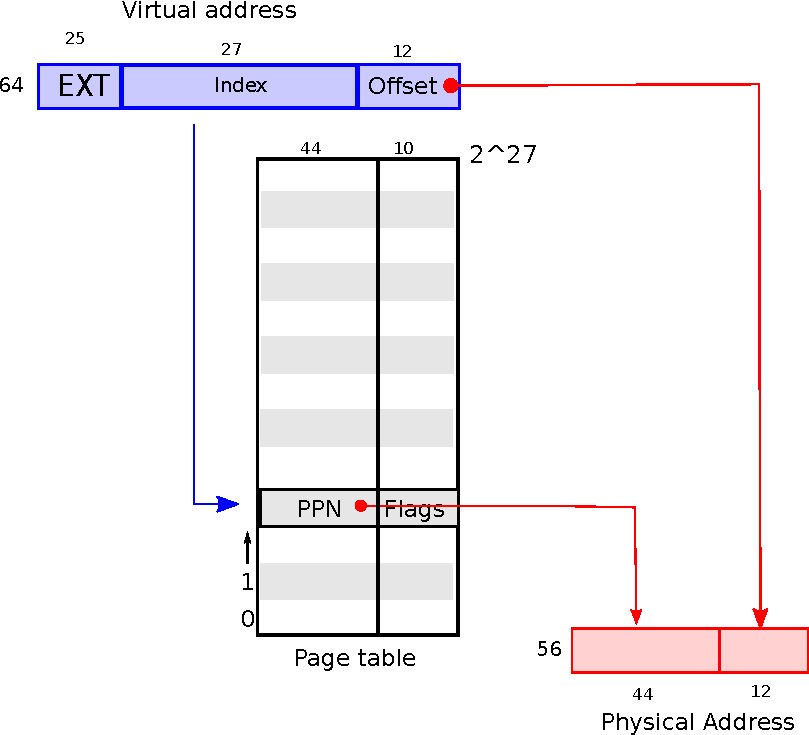
\includegraphics[scale=0.5]{fig/riscv_address.pdf}
\caption{RISC-V virtual and physical addresses, with a simplified
logical page table.}
\label{fig:riscv_address}
\end{figure}

xv6 runs on Sv39 RISC-V, which has 39-bit virtual
addresses. The top 25 bits of a
64-bit virtual address are unused.  In this Sv39 configuration, a
RISC-V page table is logically an array of $2^{27}$ (134,217,728)
\indextext{page table entries (PTEs)}.  Each PTE contains a 44-bit
physical page number (PPN) and some flags. The paging hardware
translates a virtual address by using the top 27 bits of the 39 bits
to index into the page table to find a PTE, and making a 56-bit
physical address whose top 44 bits come from the PPN in the PTE
and whose bottom 12 bits are copied from the original virtual address.
Figure~\ref{fig:riscv_address} shows this
process with a logical view of the page table as a simple array of PTEs
(see Figure~\ref{fig:riscv_pagetable} for a fuller story).
A page table
gives the operating system control over virtual-to-physical address
translations at the granularity of aligned chunks of 4096 ($2^{12}$)
bytes.  Such a chunk is called a \indextext{page}.

\begin{figure}[t]
\center
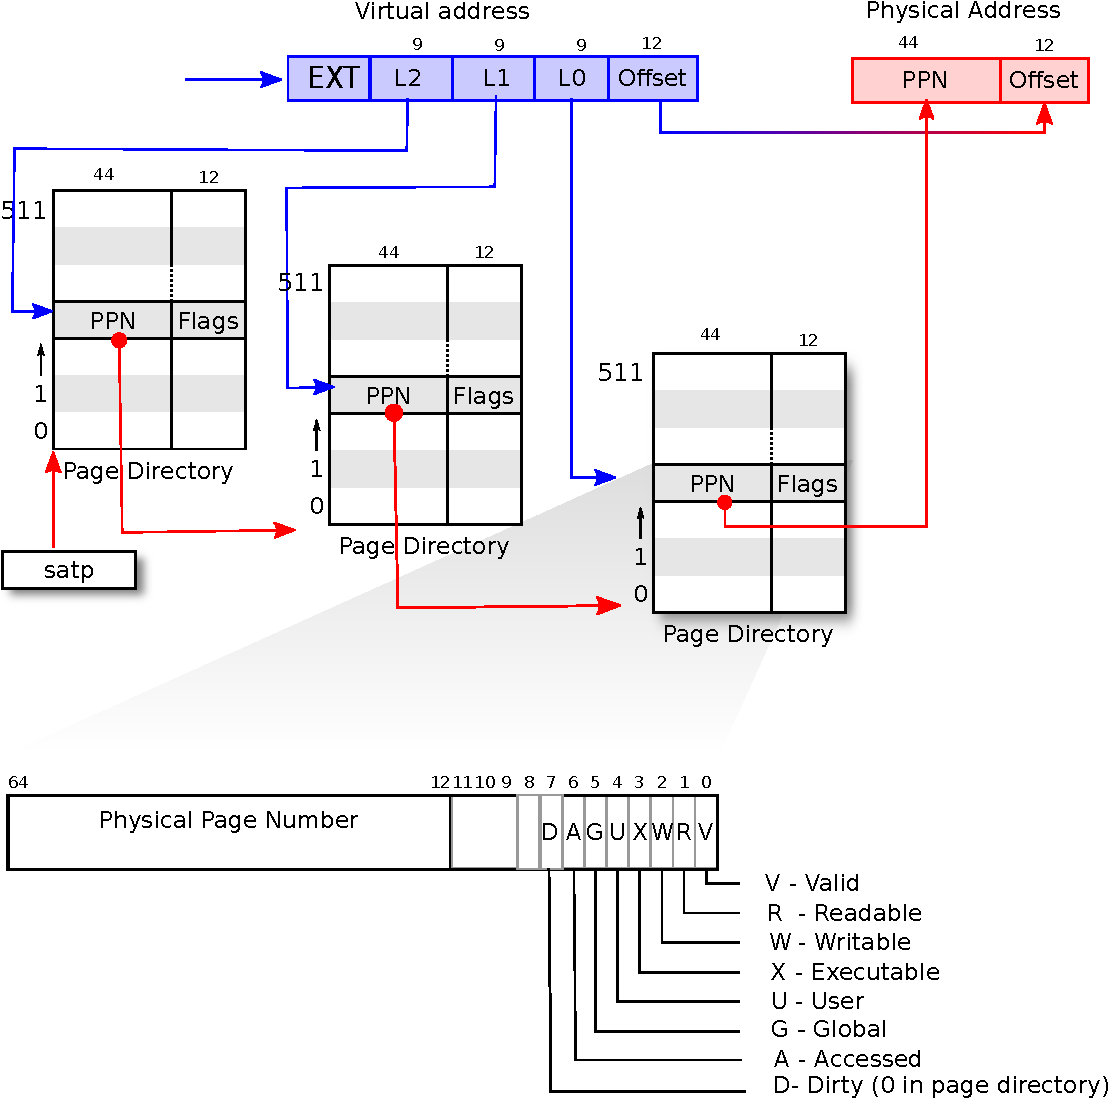
\includegraphics[scale=0.5]{fig/riscv_pagetable.pdf}
\caption{RISC-V address translation details.}
\label{fig:riscv_pagetable}
\end{figure}

In Sv39 RISC-V, the top 25 bits of a virtual address are not
used for translation; in the future, RISC-V may use those bits to
define more levels of translation.  Similarly, the physical address
has room for growth; in Sv39 it is 56 bits, but could grow to 64 bits.

As 
Figure~\ref{fig:riscv_pagetable} shows,
the actual translation happens in three steps.  A page table is stored
in physical memory as a three-level tree.
The root of the tree is a
4096-byte page-table page that contains 512 PTEs, which contain the physical
addresses for page-table pages in the next level of the tree.  Each of those
pages contains 512 PTEs for the final level in the tree.  The paging
hardware uses the top 9 bits of the 27 bits to select a PTE in the
root page-table page, the middle 9 bits to select a PTE in a page-table page in the
next level of the
tree, and the bottom 9 bits to select the final PTE.

If any of the three PTEs required to translate an address
is not present, the paging hardware raises a \indextext{page-fault exception}, leaving it up
to the kernel to handle the exception (see Chapter~\ref{CH:TRAP}).
This three-level structure allows a page table to omit entire page
table pages in the common case in which large ranges of virtual
addresses have no mappings.

Each PTE contains flag bits that tell the paging hardware
how the associated virtual address is allowed to be used.
\indexcode{PTE_V}
indicates whether the PTE is present: if it is
not set, a reference to the page causes an exception (i.e. is not allowed).
\indexcode{PTE_R}
controls whether instructions are allowed to 
read to the page.
\indexcode{PTE_W}
controls whether instructions are allowed to 
write to the page.
\indexcode{PTE_X}
controls whether the CPU may interpret the content
of the page as instructions and execute them.
\indexcode{PTE_U}
controls whether instructions in user mode are allowed
to access the page;
if \indexcode{PTE_U} is not set, the PTE can be used only in supervisor mode.
Figure~\ref{fig:riscv_pagetable}
shows how it all works.
The flags and all other page hardware-related structures are defined in
\fileref{kernel/riscv.h}

To tell the hardware to use a page table, the kernel must
write the physical address of the root page-table page into the 
\texttt{satp}\index{satp@\lstinline{satp}} register.
Each CPU has its own
\texttt{satp}.
A CPU will translate all addresses generated by subsequent instructions
using the page table pointed to by its own \texttt{satp}.
Each CPU has its own \texttt{satp} so that different CPUs can run
different processes, each with a private address space described by
its own page table.

A few notes about terms.
Physical memory refers to storage cells in DRAM.
A byte of physical memory has an address, called a physical address.
Instructions use only virtual addresses, which the
paging hardware translates to physical addresses, and then
sends to the DRAM hardware to read or write storage.
Unlike physical memory and virtual addresses, virtual memory isn't a physical object, but refers to the collection of abstractions and mechanisms
the kernel provides to manage physical memory and virtual
addresses.

\begin{figure}[h]
\centering
 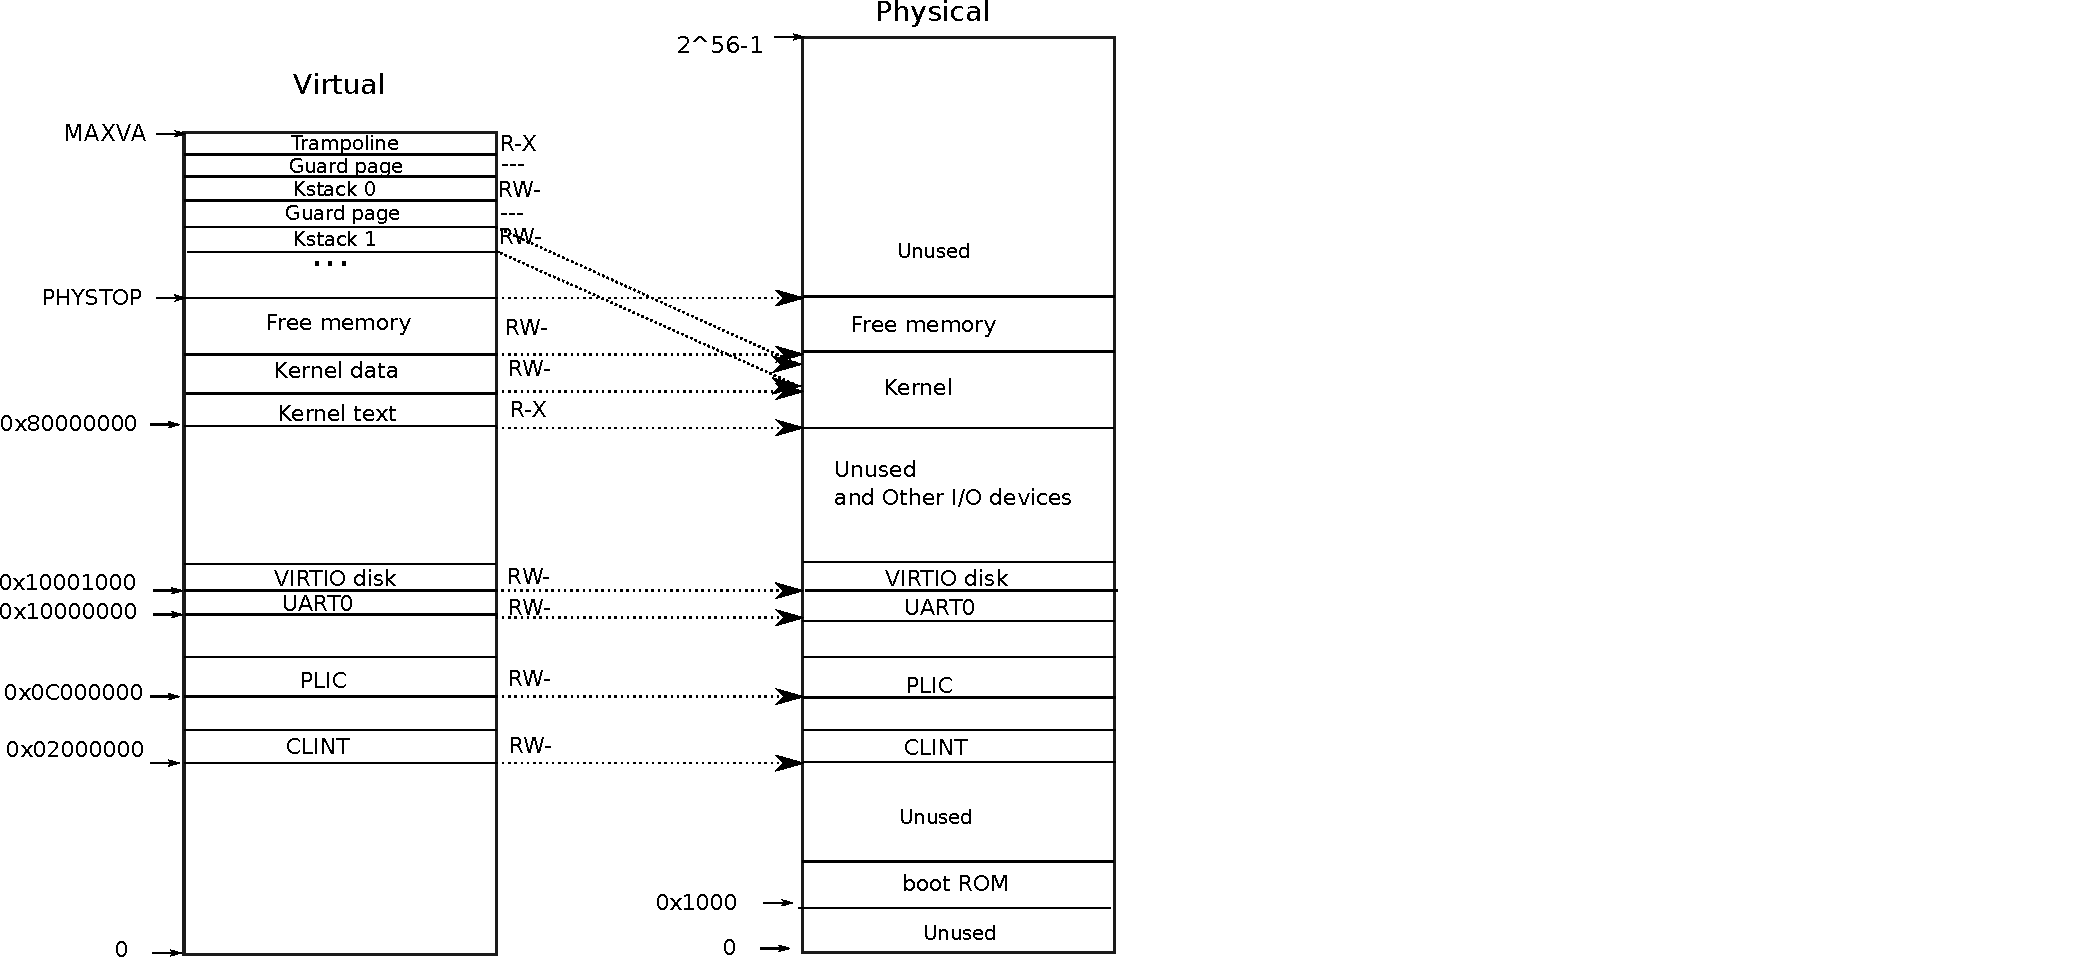
\includegraphics[scale=0.65]{fig/xv6_layout.pdf}
\caption{On the left, xv6's kernel address space.
{\sf \small{RWX}}
refer to PTE read, write, and execute permissions.
On the right, the RISC-V physical address space that
xv6 expects to see.}
\label{fig:xv6_layout}
\end{figure}

%% 
\section{Kernel address space}
%% 
The kernel has its own page table.  When a process enters the kernel,
xv6 switches to the kernel page table, and when the kernel
returns to user space, it switches to the page table of the user
process.  The memory of the kernel is private.

Figure~\ref{fig:xv6_layout}
shows the layout of the kernel address space, and the mapping from
virtual addresses to physical addresses.  The file
\fileref{kernel/memlayout.h}
declares the constants for xv6's kernel memory layout.

QEMU simulates a computer that includes I/O devices
such as a disk interface.
QEMU exposes the device interfaces to software as
\indextext{memory-mapped}
control registers that sit below
\texttt{0x80000000}
in physical memory.
The kernel can interact with the devices by reading/writing
these memory locations.
Chapter~\ref{CH:TRAP} explains
how xv6 interacts with devices.

The kernel uses an identity mapping for most virtual addresses; that
is, most of the kernel's address space is ``direct-mapped.'' For
example, the kernel itself is located at \lstinline{KERNBASE} in both
the virtual address space and in physical memory. This direct mapping
simplifies kernel code that needs to both read or write a page (with
its virtual address) and also manipulate a PTE that refers to the same
page (with its physical address). There are a couple of virtual
addresses that aren't direct-mapped:

\begin{itemize}
  
\item The trampoline page. It is mapped at the top of the virtual
  address space; user page tables have this same mapping.  In
  Chapter~\ref{CH:TRAP}, we will discuss the role of the trampoline
  page, but we see here an interesting use case of page tables; a
  physical page (holding the trampoline code) is mapped twice in the
  virtual address space of the kernel: once at top of the virtual
  address space and once in the kernel text.

\item The kernel stack pages.  Each process has its own kernel stack,
  which is mapped high so that below it xv6 can leave an unmapped \indextext{guard
    page}.  The guard page's PTE is invalid (i.e.,
  \lstinline{PTE_V} is not set), which ensures that if the kernel overflows
  a kernel stack, it will likely cause an exception and the kernel will panic.
  Without a guard page an overflowing stack would overwrite other kernel memory,
  resulting in incorrect operation. A panic crash is preferable.

\end{itemize}

While the kernel uses its stacks via the high-memory mappings, they
are also accessible to the kernel through a direct-mapped address. An
alternate design might have just the direct mapping, and use the
stacks at the direct-mapped address. In that arrangement, however,
providing guard pages would involve unmapping virtual addresses that
would otherwise refer to physical memory, which would then be hard to
use.

The kernel maps the pages for the trampoline and the kernel text with
the permissions
\lstinline{PTE_R}
and
\lstinline{PTE_X}.
The kernel reads and executes instructions from these pages.
The kernel maps the other pages with the permissions
\lstinline{PTE_R}
and
\lstinline{PTE_W},
so that it can read and write the memory in those pages.
The mappings for the guard pages are invalid.


%% 
\section{Code: creating an address space}
%% 

Most of the xv6 code for manipulating address spaces and
page tables resides in {\tt vm.c}
\lineref{kernel/vm.c:1}.
The central data structure is {\tt pagetable\_t}, which
is really a pointer to a RISC-V root page-table page;
a {\tt pagetable\_t} may be either the kernel
page table, or one of the per-process page tables.
The central functions are {\tt walk},
which finds the PTE for a virtual address,
and {\tt mappages}, which installs PTEs for new mappings.
Functions starting with {\tt kvm} manipulate
the kernel page table; functions starting with {\tt uvm}
manipulate a user page table; other functions are
used for both.
{\tt copyout} and {\tt copyin} copy data to and from
user virtual addresses provided as system call arguments;
they are in {\tt vm.c} because they need to explicitly
translate those addresses in order to find the corresponding
physical memory.

Early in the boot sequence,
\indexcode{main}
calls
\indexcode{kvminit}
\lineref{kernel/vm.c:/^kvminit/}
to create the kernel's page table.
This call occurs before xv6 has enabled paging on the RISC-V,
so addresses refer directly to physical memory.
\lstinline{Kvminit}
first allocates a page of physical memory to hold the root page-table page.
Then it calls
\indexcode{kvmmap}
to install the translations that the kernel needs.
The translations include the kernel's
instructions and data, physical memory up to
\indexcode{PHYSTOP},
and memory ranges which are actually devices.

\indexcode{kvmmap} 
\lineref{kernel/vm.c:/^kvmmap/}
calls
\indexcode{mappages}
\lineref{kernel/vm.c:/^mappages/},
which
installs mappings into a page table
for a range of virtual addresses to
a corresponding range of physical addresses.
It does this separately for each virtual address in the range,
at page intervals.
For each virtual address to be mapped,
\lstinline{mappages}
calls
\indexcode{walk}
to find the address of the PTE for that address.
It then initializes the PTE to hold the relevant physical page
number, the desired permissions 
(\lstinline{PTE_W},
\lstinline{PTE_X},
and/or
\lstinline{PTE_R}),
and
\lstinline{PTE_V}
to mark the PTE as valid
\lineref{kernel/vm.c:/perm...PTE_V/}.

\indexcode{walk}
\lineref{kernel/vm.c:/^walk/}
mimics the RISC-V paging hardware as it
looks up the PTE for a virtual address (see
Figure~\ref{fig:riscv_pagetable}).
\lstinline{walk}
descends the 3-level page table 9 bits at the time.
It uses each level's 9 bits of virtual address to find
the PTE of either the next-level page table or the final page
\lineref{kernel/vm.c:/pte.=..pagetable/}.
If the PTE isn't valid, then
the required page hasn't yet been allocated;
if the
\lstinline{alloc}
argument is set,
\lstinline{walk}
allocates a new page-table page and puts its physical address in the PTE.
It returns the address of the PTE in the lowest layer in the tree
\lineref{kernel/vm.c:/return..pagetable/}.

The above code depends on physical memory being direct-mapped into the
kernel virtual address space. For example, as \lstinline{walk} descends levels
of the page table, it pulls the (physical) address of the
next-level-down page table from a PTE \lineref{kernel/vm.c:/pagetable.=..pa.*E2P/},
and then uses that address as a
virtual address to fetch the PTE at the next level down
\lineref{kernel/vm.c:/t..pte.=..paget/}.

\indexcode{main}
calls
\indexcode{kvminithart}
\lineref{kernel/vm.c:/^kvminithart/}
to install the kernel page table.
It writes the physical address of the root page-table page
into the register
\texttt{satp}.
After this the CPU will translate addresses using the kernel
page table.  Since the kernel uses an identity mapping, the now
virtual address of the next instruction will map to the right physical
memory address.

\indexcode{procinit} \lineref{kernel/proc.c:/^procinit/}, which is
called from \lstinline{main}, allocates a kernel stack for each
process. It maps each stack at the virtual address generated by
\lstinline{KSTACK}, which leaves room for the invalid stack-guard
pages. \lstinline{kvmmap} adds the mapping PTEs to the kernel page
table, and the call to \lstinline{kvminithart} reloads the kernel page
table into \texttt{satp} so that the hardware knows about the new
PTEs.

Each RISC-V CPU caches page table entries in a
\indextext{Translation Look-aside Buffer (TLB)}, and when xv6 changes
a page table, it must tell the CPU to invalidate corresponding
cached TLB entries.  If it didn't,
then at some point later the TLB might
use an old cached mapping, pointing to a physical page that in the meantime
has been allocated to another process, and as a result, a process
might be able to scribble on some other process's memory.  The RISC-V
has an instruction \indexcode{sfence.vma} that flushes
the current CPU's TLB.
xv6 executes {\tt sfence.vma} in {\tt kvminithart}  after reloading the 
\texttt{satp} register, and in the trampoline code that
switches to a user page table before returning to user space
\lineref{kernel/trampoline.S:/sfence.vma/}.

\section{Physical memory allocation}

The kernel must allocate and free physical memory at run-time for
page tables,
user memory,
kernel stacks,
and pipe buffers.

xv6 uses the physical memory between the end of the kernel and
\indexcode{PHYSTOP}
for run-time allocation. It allocates and frees whole 4096-byte pages
at a time. It keeps track of which pages are free by threading a
linked list through the pages themselves. Allocation consists of
removing a page from the linked list; freeing consists of adding the
freed page to the list.
%% 
\section{Code: Physical memory allocator}
%% 

The allocator resides in {\tt kalloc.c} \lineref{kernel/kalloc.c:1}.
The allocator's data structure is a
\textit{free list}
of physical memory pages that are available
for allocation.
Each free page's list element is a
\indexcode{struct run}
\lineref{kernel/kalloc.c:/^struct.run/}.
Where does the allocator get the memory
to hold that data structure?
It store each free page's
\lstinline{run}
structure in the free page itself,
since there's nothing else stored there.
The free list is
protected by a spin lock
\linerefs{kernel/kalloc.c:/^struct.{/,/}/}.
The list and the lock are wrapped in a struct
to make clear that the lock protects the fields
in the struct.
For now, ignore the lock and the calls to
\lstinline{acquire}
and
\lstinline{release};
Chapter~\ref{CH:LOCK} will examine
locking in detail.

The function
\indexcode{main}
calls
\indexcode{kinit}
to initialize the allocator
\lineref{kernel/kalloc.c:/^kinit/}.
\lstinline{kinit}
initializes the free list to hold
every page between the end of the kernel and {\tt PHYSTOP}.
\lstinline{xv6}
ought to determine how much physical
memory is available by parsing configuration information that
is provide by the hardware.
Instead xv6 assumes that the machine has
128 megabytes of RAM.
\lstinline{kinit}
calls
\indexcode{freerange}
to add memory to the free list via per-page calls to
\indexcode{kfree}.
A PTE can only refer to a physical address that is aligned
on a 4096-byte boundary (is a multiple of 4096), so
\lstinline{freerange}
uses
\indexcode{PGROUNDUP}
to ensure that it frees only aligned physical addresses.
The allocator starts with no memory;
these calls to
\lstinline{kfree}
give it some to manage.

The allocator sometimes treats addresses as integers
in order to perform arithmetic on them (e.g.,
traversing all pages in
\lstinline{freerange}),
and sometimes uses addresses as pointers to read and
write memory (e.g., manipulating the
\lstinline{run}
structure stored in each page);
this dual use of addresses is the main reason that the
allocator code is full of C type casts.
\index{type cast}
The other reason is that freeing and allocation inherently
change the type of the memory.

The function
\lstinline{kfree}
\lineref{kernel/kalloc.c:/^kfree/}
begins by setting every byte in the
memory being freed to the value 1.
This will cause code that uses memory after freeing it
(uses ``dangling references'')
to read garbage instead of the old valid contents;
hopefully that will cause such code to break faster.
Then
\lstinline{kfree}
prepends the page to the free list:
it casts
\lstinline{pa}
to a pointer to
\lstinline{struct}
\lstinline{run},
records the old start of the free list in
\lstinline{r->next},
and sets the free list equal to
\lstinline{r}.
\indexcode{kalloc}
removes and returns the first element in the free list.

\section{Process address space}

Each process has a separate page table, and when xv6 switches between
processes, it also changes page tables.
As 
Figure~\ref{fig:as} shows,
a process's user memory starts at virtual address
zero and can grow up to
\texttt{MAXVA}
\lineref{kernel/riscv.h:/MAXVA/},
allowing a process to address in principle 256 Gigabytes of memory.

When a process asks xv6 for more user memory,
xv6 first uses {\tt kalloc} to allocate physical pages.
It then adds PTEs to the process's page table that point
to the new physical pages.
Xv6 sets the
\lstinline{PTE_W},
\lstinline{PTE_X},
\lstinline{PTE_R},
\lstinline{PTE_U},
and
\lstinline{PTE_V}
flags in these PTEs.
Most processes do not use the entire user address space;
xv6 leaves
\lstinline{PTE_V}
clear in unused PTEs.

We see here a few nice examples of use of page tables.  First,
different processes' page tables translate user addresses to different
pages of physical memory, so that each process has private user
memory.  Second, each process sees its memory as having contiguous
virtual addresses starting at zero, while the process's physical
memory can be non-contiguous.  Third, the kernel maps a page with
trampoline code at the top of
the user address space, thus a single page of physical memory
shows up in all address spaces.

\begin{figure}[t]
\center
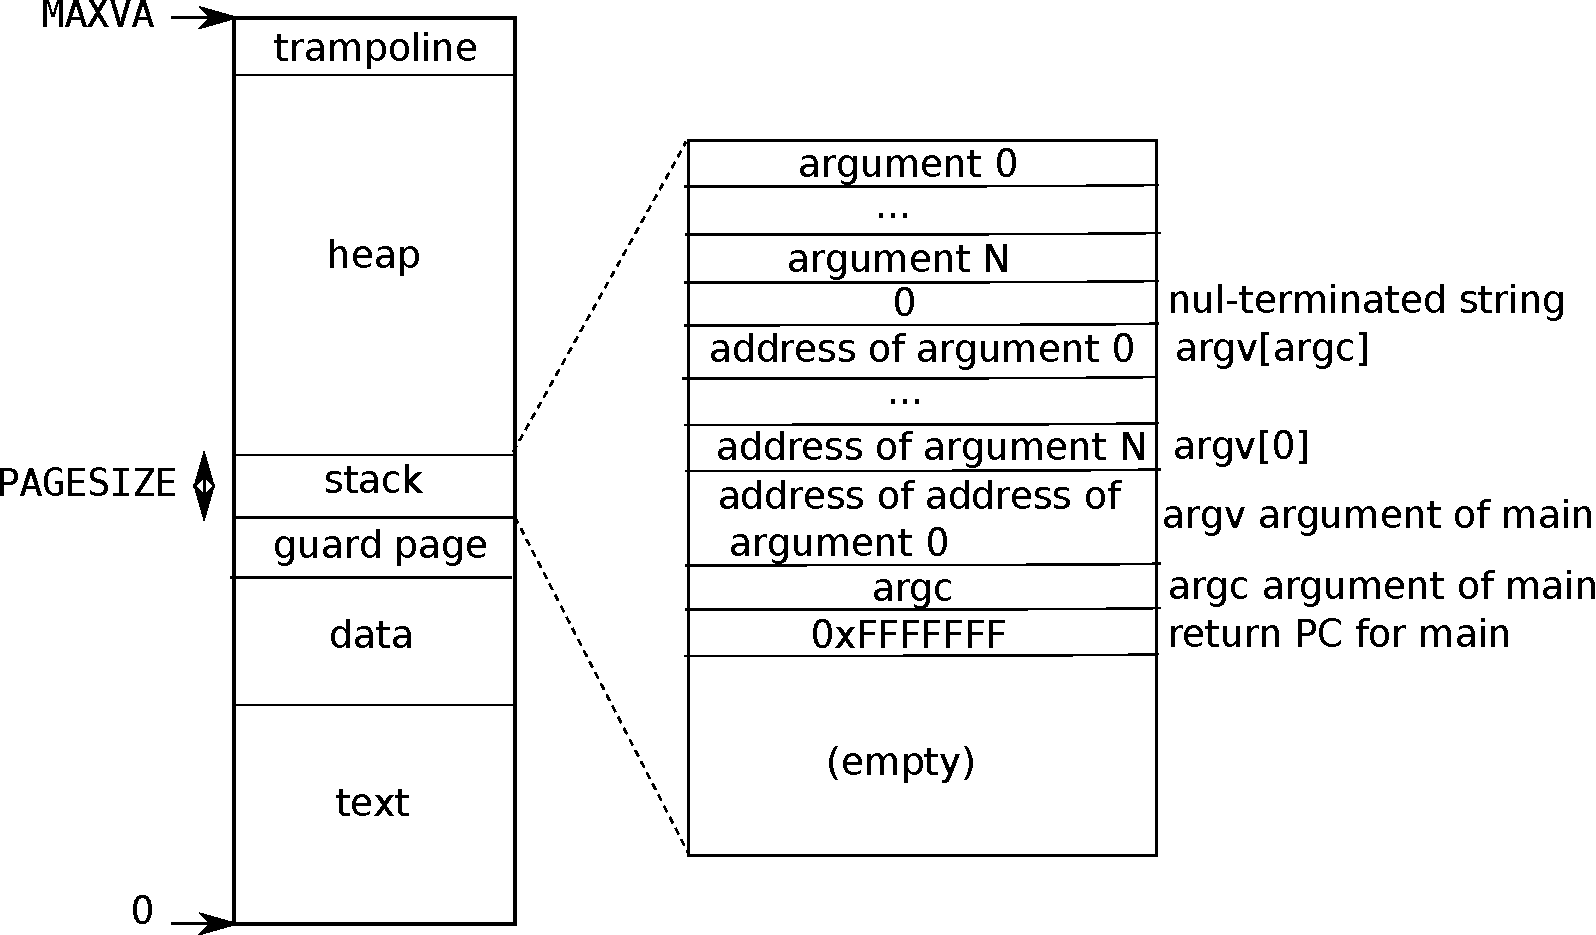
\includegraphics[scale=0.5]{fig/processlayout.pdf}
\caption{A process's user address space, with its initial stack.}
\label{fig:processlayout}
\end{figure}

Figure~\ref{fig:processlayout} shows the layout of the user memory of
an executing process in xv6 in more detail.  The stack is a single
page, and is shown with the initial contents as created by exec.
Strings containing the command-line arguments, as well as an array of
pointers to them, are at the very top of the stack.  Just under that
are values that allow a program to start at \lstinline{main} as if the
function \lstinline{main(argc}, \lstinline{argv)} had just
been called.

To detect a user stack overflowing the allocated stack memory, xv6
places an invalid guard page right below the stack. If the user stack
overflows and the process tries to use an address below the stack, the
hardware will generate a page-fault exception because the mapping is
not valid. A real-world operating system might instead automatically
allocate more memory for the user stack when it overflows.

\section{Code: sbrk}

\lstinline{Sbrk}
is the system call for a process to shrink or grow its memory. The system
call is implemented by the function
\lstinline{growproc}
\lineref{kernel/proc.c:/^growproc/}.
\lstinline{growproc} calls \lstinline{uvmalloc} or
\lstinline{uvmdealloc}, depending on whether \lstinline{n} is postive
or negative.
\lstinline{uvmalloc}
\lineref{kernel/vm.c:/^uvmalloc/}
allocates physical memory with {\tt kalloc},
and adds PTEs to the user page table with {\tt mappages}.
\lstinline{uvmdealloc} calls
{\tt uvmunmap}
\lineref{kernel/vm.c:/^uvmunmap/},
which uses {\tt walk} to find PTEs and
{\tt kfree} to free the physical memory they refer to.

xv6 uses a process's page table not just to tell the hardware how to
map user virtual addresses, but also as the only record of which
physical memory pages are allocated to that process. That is the
reason why freeing user memory (in {\tt uvmunmap}) requires
examination of the user page table.

%% 
\section{Code: exec}
%% 
\lstinline{Exec}
is the system call that creates the user part of an address space.  It
initializes the user part of an address space from a file stored in the file
system.
\lstinline{Exec}
\lineref{kernel/exec.c:/^exec/}
opens the named binary
\lstinline{path}
using
\indexcode{namei}
\lineref{kernel/exec.c:/namei/},
which is explained in Chapter~\ref{CH:FS}.
Then, it reads the ELF header. Xv6 applications are described in the widely-used
\indextext{ELF format},
defined in
\fileref{kernel/elf.h}.
An ELF binary consists of an ELF header,
\indexcode{struct elfhdr}
\lineref{kernel/elf.h:/^struct.elfhdr/},
followed by a sequence of program section headers,
\lstinline{struct proghdr}
\lineref{kernel/elf.h:/^struct.proghdr/}.
Each
\lstinline{proghdr}
describes a section of the application that must be loaded into memory;
xv6 programs have only one program section header, but
other systems might have separate sections
for instructions and data.

The first step is a quick check that the file probably contains an
ELF binary.
An ELF binary starts with the four-byte ``magic number''
\lstinline{0x7F},
\lstinline{`E'},
\lstinline{`L'},
\lstinline{`F'},
or
\indexcode{ELF_MAGIC}
\lineref{kernel/elf.h:/ELF_MAGIC/}.
If the ELF header has the right magic number,
\lstinline{exec}
assumes that the binary is well-formed.

\lstinline{Exec}
allocates a new page table with no user mappings with
\indexcode{proc_pagetable}
\lineref{kernel/exec.c:/proc_pagetable/},
allocates memory for each ELF segment with
\indexcode{uvmalloc}
\lineref{kernel/exec.c:/uvmalloc/},
and loads each segment into memory with
\indexcode{loadseg}
\lineref{kernel/exec.c:/loadseg/}.
\lstinline{loadseg}
uses
\indexcode{walkaddr}
to find the physical address of the allocated memory at which to write
each page of the ELF segment, and
\indexcode{readi}
to read from the file.

The program section header for
\indexcode{/init},
the first user program created with
\lstinline{exec},
looks like this:
\begin{footnotesize}
\begin{verbatim}
# objdump -p _init
user/_init:     file format elf64-littleriscv

Program Header:
    LOAD off    0x00000000000000b0 vaddr 0x0000000000000000 
                                      paddr 0x0000000000000000 align 2**3
         filesz 0x0000000000000840 memsz 0x0000000000000858 flags rwx
   STACK off    0x0000000000000000 vaddr 0x0000000000000000 
                                      paddr 0x0000000000000000 align 2**4
         filesz 0x0000000000000000 memsz 0x0000000000000000 flags rw-
\end{verbatim}
\end{footnotesize}

The program section header's
\lstinline{filesz}
may be less than the
\lstinline{memsz},
indicating that the gap between them should be filled
with zeroes (for C global variables) rather than read from the file.
For
\lstinline{/init},
\lstinline{filesz}
is 2112 bytes and
\lstinline{memsz}
is 2136 bytes,
and thus
\indexcode{uvmalloc}
allocates enough physical memory to hold 2136 bytes, but reads only 2112 bytes
from the file
\lstinline{/init}.

Now
\indexcode{exec}
allocates and initializes the user stack.
It allocates just one stack page.
\lstinline{Exec}
copies the argument strings to the top of the stack
one at a time, recording the pointers to them in
\indexcode{ustack}.
It places a null pointer at the end of what will be the
\indexcode{argv}
list passed to
\lstinline{main}.
The first three entries in
\lstinline{ustack}
are the fake return program counter,
\indexcode{argc},
and
\lstinline{argv}
pointer.

\lstinline{Exec}
places an inaccessible page just below the stack page,
so that programs that try to use more than one page will fault.
This inaccessible page also allows
\lstinline{exec}
to deal with arguments that are too large;
in that situation,
the
\indexcode{copyout}
\lineref{kernel/vm.c:/^copyout/}
function that
\lstinline{exec}
uses to copy arguments to the stack will notice that
the destination page is not accessible, and will
return -1.

During the preparation of the new memory image,
if
\lstinline{exec}
detects an error like an invalid program segment,
it jumps to the label
\lstinline{bad},
frees the new image,
and returns -1.
\lstinline{Exec}
must wait to free the old image until it
is sure that the system call will succeed:
if the old image is gone,
the system call cannot return -1 to it.
The only error cases in
\lstinline{exec}
happen during the creation of the image.
Once the image is complete,
\lstinline{exec}
can commit to the new page table
\lineref{kernel/exec.c:/pagetable.=.pagetable/}
and free the old one
\lineref{kernel/exec.c:/proc_freepagetable/}.

\lstinline{Exec}
loads bytes from the ELF file into memory at addresses specified by the ELF file.
Users or processes can place whatever addresses they want into an ELF file.
Thus
\lstinline{exec}
is risky, because the addresses in the ELF file may refer to the kernel, accidentally
or on purpose. The consequences for an unwary kernel could range from
a crash to a malicious subversion of the kernel's isolation mechanisms
(i.e., a security exploit).
xv6 performs a number of checks to avoid these risks.
For example
\lstinline{if(ph.vaddr + ph.memsz < ph.vaddr)}
checks for whether the sum overflows a 64-bit integer.
The danger is that a user could construct an ELF binary with a
\lstinline{ph.vaddr}
that points to a user-chosen address,
and
\lstinline{ph.memsz}
large enough that the sum overflows to 0x1000, which will look like a
valid value. In an older version of xv6 in which the user address
space also contained the kernel (but not readable/writable in user
mode), the user could choose an address that corresponded to kernel
memory and would thus copy data from the ELF binary into the kernel.
In the RISC-V version of xv6 this cannot happen, because the kernel has
its own separate page table;
\lstinline{loadseg}
loads into the process's page table, not in the kernel's page table.

It is easy for a kernel developer to omit a crucial check, and
real-world kernels have a long history of missing checks whose absence
can be exploited by user programs to obtain kernel privileges.  It is likely that xv6 doesn't do a complete job of validating
user-level data supplied to the kernel, which a malicious user program might be able to exploit to circumvent xv6's isolation.
%% 
\section{Real world}
%% 

Like most operating systems, xv6 uses the paging hardware for memory
protection and mapping.  Most operating systems make far more
sophisticated use of paging than xv6 by combining paging and
page-fault exceptions, which we will discuss in
Chapter~\ref{CH:TRAP}.

RISC-V supports protection at the level of physical addresses,
but xv6 doesn't use that feature.

On machines with lots of memory
it might make sense to use
RISC-V's support for ``super pages.''
Small pages make sense
when physical memory is small, to allow allocation and page-out to disk
with fine granularity.
For example, if a program
uses only 8 kilobytes of memory, giving it a whole 4-megabyte super-page
of physical memory is wasteful.
Larger pages make sense on machines with lots of RAM,
and may reduce overhead for page-table manipulation.

The xv6 kernel's lack of a {\tt malloc}-like allocator that can
provide memory for small objects prevents the kernel from using
sophisticated data structures that would require dynamic allocation.

Memory allocation was a hot topic a long time ago, the basic problems being
efficient use of limited memory and
preparing for unknown future requests~\cite{knuth}.  Today people care more about speed than
space efficiency.  In addition, a more elaborate kernel
would likely allocate many different sizes of small blocks,
rather than (as in xv6) just 4096-byte blocks;
a real kernel
allocator would need to handle small allocations as well as large
ones.
%% 
\section{Exercises}
%% 

\begin{enumerate}
  
\item Parse RISC-V's device tree to find the amount of physical memory
the computer has.

\item Write a user program that grows its address space by one byte by calling
\lstinline{sbrk(1)}.
Run the  program and investigate the page table for the program before the call
to
\lstinline{sbrk}
and after the call to
\lstinline{sbrk}.
How much space has the kernel allocated?  What does the
\lstinline{pte}
for the new memory contain?

\item Modify xv6 to use super pages for the kernel.

\item Modify xv6 so that when a user program dereferences a null pointer, it will
receive an exception.  That is, modify xv6 so that virtual address 0 isn't mapped for
user programs.

\item Unix implementations of
\lstinline{exec}
traditionally include special handling for shell scripts.
If the file to execute begins with the text
\lstinline{#!},
then the first line is taken to be a program
to run to interpret the file.
For example, if
\lstinline{exec}
is called to run
\lstinline{myprog}
\lstinline{arg1}
and
\lstinline{myprog} 's
first line is
\lstinline{#!/interp},
then
\lstinline{exec}
runs
\lstinline{/interp}
with command line
\lstinline{/interp}
\lstinline{myprog}
\lstinline{arg1}.
Implement support for this convention in xv6.

\item Implement address space randomization for the kernel.

\end{enumerate}

